\chapter{Complexity System}
\section{Grey System}
灰色系统理论(Grey System Theory, GS)\cite{deng1982control,deng1986grey,deng1987basic,deng1989introduction,deng2005primary}由华中科技大学教授邓聚龙于1982年提出,是处理少数据不确定性问题的理论。

灰色系统理论主要通过对“部分”已知信息的生成、开发,提取有价值的信息,实现对系统运行行为、演化规律的正确描述和有效监控。在灰色系统理论中,少数据不确定性又称为灰性,并称具有灰性的系统为\textbf{灰色系统},信息完全的系统为\textbf{白色系统},反之信息缺乏的系统称为\textbf{黑色系统}。人体就是一个灰色系统,尽管人体的部分外部参数,如身高、体重等及部分内部参数,如体温、血压等是已知的,但更多的参数是未知的。除人体之外,工业、 农业、 社会经济等领域,由于运行机制不清晰,环境变化,条件复杂,处理手段有限等,有许多的系统呈现灰性\cite{deng1987grey}\footnote{\href{http://61.133.8.10:8080/date\%5CN\%5CA2087467.pdf}{灰色系统基本方法}}。

迄今为止,灰色系统理论已经成功应用于医学、图像处理、机器人、工业技术、股票价格预测\cite{wang2002predicting}、时间序列分析\cite{kayacan2010grey}等方面,并取得实效。

\section{Membrane Computing/P System}
生物细胞可以生长、分裂、对刺激产生反应、产生一系列的化学反应,是一种典型的功能复杂又健壮无比的系统。自然计算是信息科学的一个分支,意图根据生物系统的结构和功能,寻求新的解决问题的思路,抽象出新的计算模型。比如,神经网络(Neural Network)、进化计算(Evolutionary Computing)、群体智能(Swarm Intelligence)、DNA计算(DNA Computing)都属于自然计算,模仿生物系统而构造的计算模型。

\begin{figure}[htbp]
\begin{minipage}[t]{0.49\linewidth}
\centering
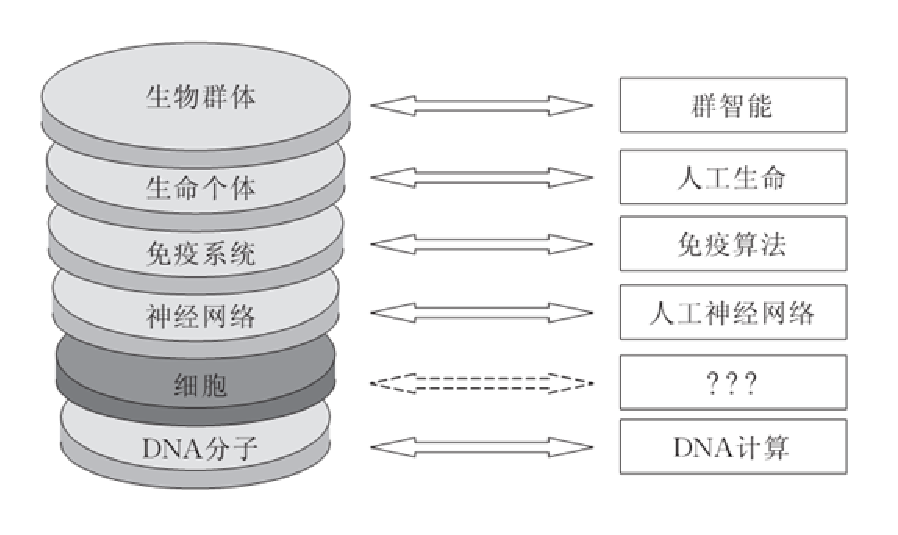
\includegraphics[width=0.8\textwidth, height=8cm]{figures/naturecompute.eps}
\caption{Nature Computing\cite{zhang2010nature}}
\end{minipage}
\begin{minipage}[t]{0.49\linewidth}
\centering
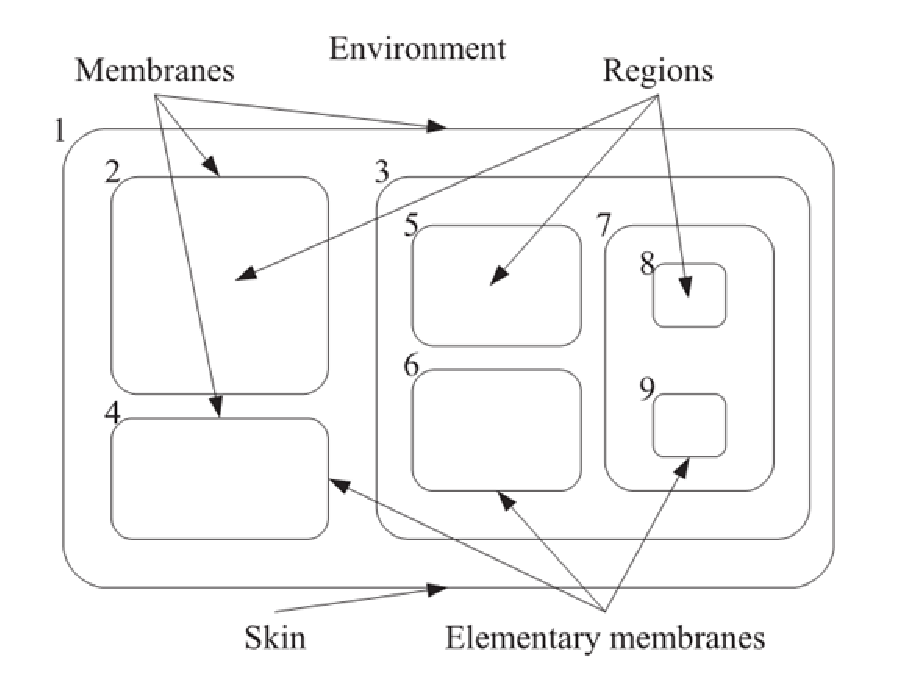
\includegraphics[width=0.8\textwidth, height=8cm]{figures/membrane.eps}
\caption{A typical membrane structure of a P system\cite{buiu2012development}}
\label{fig:membrane}
\end{minipage}
\end{figure}

膜计算(Membrane Computing)是由P{\u{a}}un于2000年提出\cite{paun2000computing},历经十多年的发展,已经成为一个新兴的研究领域。出于对P{\u{a}}un的尊重,膜计算还有一个更有名的称谓——P系统(P System, PS)。

PS是基于真核细胞(Eukaryotic Cell)结构,模仿生物膜系统中化学物质的化学反应行为,抽象出来的计算模型。P系统的结构(膜结构)是一种膜的层次排列,如图\ref{fig:membrane}所示,最外层膜1称作表层膜,将系统及其周围环境分隔。膜2和4因为不包含其他膜,称为基本膜(Elementary Membrane)。每层膜所包围的部分称作区域(Region),区域由对象的多重集(Multiset)和进化规则(Evolution Rule)构成,通常从初始状态(多重集)开始,按照进化规则执行计算。

PS已经应用到多个领域,如生物、生物医学、计算机图形学、语言学、经济学、计算机科学和密码学等\cite{zhang2010nature}。

\section{膜系统的设计}
尽管PS可以为研究人员提供各种解决方案,设计出合理的膜系统却并非易事。Gabriela等人\cite{escuela2010application}提出使用遗传算法进化PS,无需人工过多干预即可完成进化。Huang等人\cite{huang2012evolutionary}提出配置量子启发式进化算法(Quantum-Inspired Evolutionary Algorithm,QIEA),基于预先定义的变量和规则,实现PS的自动设计。

关于PS的参考资料、仿真软件、有待研究的问题、会议信息和主要学者的联系方式等均可从\href{http://ppage.psystems.eu/}{The P Systems Webpage}获取。

\section{数值P系统}
数值P系统(Numerical P System, NPS)最初由P{\u{a}}un和P{\u{a}}un\cite{paun2006introduction,paun2006membrane}提出。Buiu等人\cite{buiu2011software}使用Java 语言开发了首个数值P系统模拟器(SNUPS),并使用一个微分方程示例说明SNUPS的基本功能。与PS相似,NPS 具有相同的结构,区别就是用数值变量代替了PS 的符号,每个膜都包含一个生产函数(Production Function)和一个分解规则(Repartition Protocol)。每个局部变量都有一个初始值,然后将初值带入生产函数产出数值,遵照分解规则分配给不同的膜。

NPS的计算是并发执行,在每步计算中,所有区域的生产函数都是同时执行。典型的分解规则是如下所示:
\[c_1|\nu_1 + c_2|\nu_2 + c_3|\nu_3 + \dots + c_n|\nu_n\]
其中,$c_i$表示变量$\nu_i$能够从生产值中分配到的比例,假设单位比例为$p$,那么每次计算变量$c_i$都可以分到$p*c_i$。如果某个变量存在多个分配来源,直接加总即可。

如果一个变量$x_{ij}$包含在某个生产函数中,则称它是Productive,每次计算被消耗掉以后,重置为0,否则将其加到分配的数值上。

\subsection{示例}
下图是一个简单的NPS,它包含两个膜结构。
\begin{figure}[htbp]
\centering
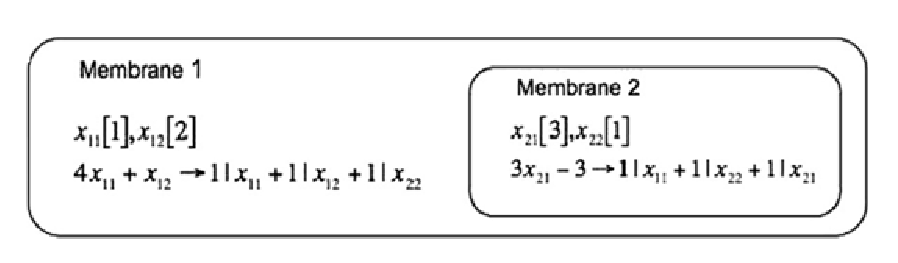
\includegraphics[width=0.8\textwidth, height=3cm]{figures/membraneinstance.eps}
\caption{示例\cite{buiu2012development}}
\end{figure}

为了说明NPS的工作机理,以下列出该NPS的2步迭代过程:
\begin{enumerate}[Step 1]
\item
\textbf{膜1}:带入初始值$x_{11}=1$,$x_{12}=2$,生产量为$F_1=4x_{11}+x_{12}=6$,按照分解规则分解,要分成3份($x_{11}$、$x_{12}$、$x_{22}$各一份),平均每份$q_1=2$。

\textbf{膜2}:带入初值$x_{21}=3$,$x_{22}=1$,生产$F_2=3x_{21}-3=6$,平均每份$q_2=2$。

\textbf{更新}:

\subitem 变量$x_{11}$是Productive:$x_{11}=1*q_1+1*q_2=2+2=4$
\subitem 变量$x_{12}$是Productive:$x_{12}=1*q_1=2$
\subitem 变量$x_{21}$是Productive:$x_{21}=1*q_2=2$
\subitem 变量$x_{22}$是Non-Productive:$x_{22}=1+1*q_1+1*q_2=1+2+2=5$

\item
\textbf{膜1}:带入初始值$x_{11}=4$,$x_{12}=2$,生产$F_1=4x_{11}+x_{12}=18$,$q_1=6$。

\textbf{膜2}:带入初值$x_{21}=2$,$x_{22}=5$,生产$F_2=3x_{21}-3=3$,平均每份$q_2=1$。

\textbf{更新}:

\subitem 变量$x_{11}$是Productive:$x_{11}=1*q_1+1*q_2=7$
\subitem 变量$x_{12}$是Productive:$x_{12}=1*q_1=6$
\subitem 变量$x_{21}$是Productive:$x_{21}=1*q_2=1$
\subitem 变量$x_{22}$是Non-Productive:$x_{22}=5+1*q_1+1*q_2=12$
\end{enumerate}

\subsection{模型}
一个NPS可以抽象为如下形式的模型:
\begin{equation}\label{eq:nps}
\Pi = (m,H,\mu, (Var_1,Pr_1,Var_1(0)),\ldots, (Var_m,Pr_m,Var_m(0)))
\end{equation}
其中:
\begin{itemize}
\item $m$是$\Pi$的度(Degree),表示系统包含的膜的个数,一般地,$m\le 1$。
\item $H$是一个包含了$m$个符号的字母表,每个符号代表一个膜。
\item $\mu$表示一个膜结构,说明系统中膜的排列形式。
\item $Var_i$是膜$i$区域内的变量集合,初始值为$Var_i(0)$。
\item $Pr_i$是膜$i$区域内处理变量的程序集合,由生产函数和分解规则组成:

\[Pr_{l,i} = (F_{l,i}(x_{1,i},\ldots,x_{k_i,i}), c_{l,1}|\nu_1 + \ldots + c_{l,n_i}|\nu_{n_i})\]
\end{itemize}

\section{Webots仿真软件}
Webots\footnote{\url{http://www.cyberbotics.com/}}是一个三维移动机器人模拟器,可用于建模、编程与模拟移动机器人的行为。研究人员可以使用Webots在同一个环境中设计出复杂的机器设备,可以包含一个或者多个、相似的或不同的机器人。每个工程的基本属性,如形状、颜色、质地、质量等都可由用户自己灵活选择。Webots 还提供了大量的传感器和驱动器(Sensor \& Actuator)可以选择转配给机器人。机器人控制器(Robot Controller)可以在内置的IDE 或第三方开发环境上编写。机器人的行为可以在现实物理环境中测试。Webots最新版本7.1.2,2013年03月11日发布。

Webots 7.0 Java API包含大约25个类,200个公用函数。使用Java编写控制器,需要导入Controller.jar包。包中的每个类代表一个场景树(Scene Tree,如Robot,LED等),后者功能(Utility,如Motion,ImageRef等),详细的介绍可以参看Webots Reference Manual或者Guide的第六章,或者源代码。

Webots同时支持Linux和Windows平台,但是对于Windows,只支持32位系统。在使用Eclipse编写Controller时,需要添加依赖的动态链接库,最粗糙的做法是将Webots下所有的dll文件放置到同一个文件夹,并添加到环境变量Path中。

\section{元胞自动机}
元胞自动机(Cellular Automaton,CA)是一种离散模型,在可算性理论、数学及理论生物学都有相关研究。元胞自动机最早是由John von Neumann在1950年代为模拟生物细胞的自我复制而提出的,但是并未受到学术界重视。直到1970年,剑桥大学的John Horton Conway设计了一个电脑游戏《生命游戏》后才吸引了科学家们的注意。此后,Stephen Wolfram对初等元胞机256种规则所产生的模型进行了深入研究,并用熵来描述其演化行为,将元胞自动机分为平稳型、周期型、混沌型和复杂型。

一个标准的元胞自动机($A$)由元胞、元胞状态、邻域和状态更新规则构成。用数学表示为:
\begin{equation}\label{eq:ca}
  A = (L, d, S, N, f)
\end{equation}
其中$L$为元胞空间,$d$为元胞自动机内元胞空间的维数,$S$是元胞有限的、离散的状态集合,$N$为某个邻域内所有元胞的集合,$f$为局部映射或局部规则。

\section{股票市场}
股票市场是一个典型的复杂系统,具有多样性,影响股票市场行情走势的因素不计其数。从长期趋势来看,股票市场的波动无章可循,如果没有海量数据分析支撑,人们对股票市场的预测就等于是随机猜测。

\subsection{Google搜索之群羊效应}
2010年,Preis等人通过分析2004年至2010年期间Google搜索引擎的搜索记录\cite{preis2010complex},发现每周标普500公司的股票交易额同人们每周向Google提交的包含标普500公司名称的检索词数量之间存在着紧密的关联,这一行为与“群羊效应”(Herd Effect)颇有相似。图\ref{eq:sp500withquery}是标普500指数与人们查询“雷曼兄弟银行”的次数之间的关系。
\begin{figure}
  \centering
  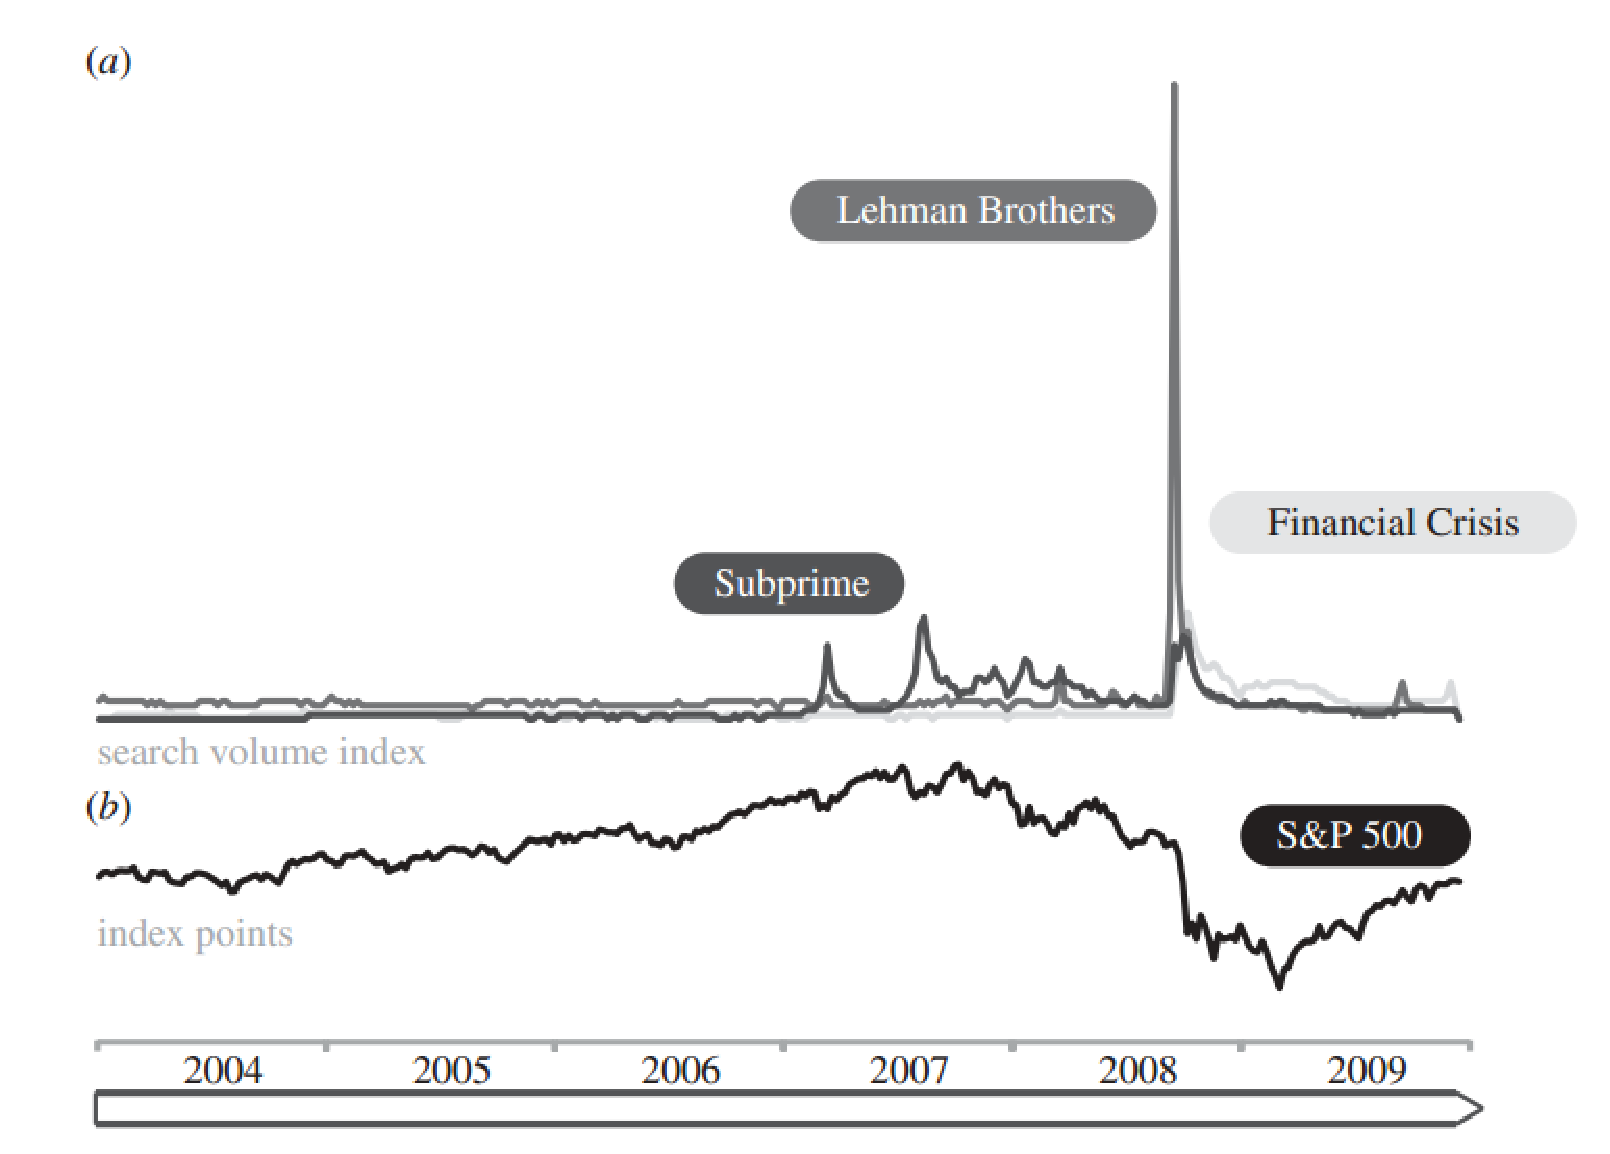
\includegraphics[width=0.85\textwidth,height=5cm]{figures/sp500withquery.eps}
  \caption{S\&P 500与S\&P 500公司查询数量之间的关系}\label{eq:sp500withquery}
\end{figure}

\subsection{社交网络之情绪集散地}
Johan Bollen等人\cite{bollen2011twitter}分析社交网络Twitter在2008年近一千万条推文,发现利用Twitter数据可以预测未来一周的股市波动趋势。他们使用两种工具追踪Twitter用户的情绪:一种是开源工具OpinionFinder,可以将推文划分为正面和负面两种情绪;一种是GPOMS(Google-Profile of Mood States),从冷静(Calm)、警惕(Alert)、确信(Sure)、活力(Vital)、友善(Kind)和幸福(Happy)六个维度来度量情绪。

为了验证两个工具的准确性,他们将Twitter用户的情绪和社会事件对比,发现结果两相吻合。例如,在总统大选日(2008年11月4日)期间,Twitter 在大选日前一天开始紧张,在大选日当天变得冷静、活力、友善、幸福,总体情绪在大选日后又回归平常。在感恩节(11月28日)当天,整个 Twitter 洋溢着浓浓的幸福味道,过后又恢复正常。最不可思议的是,将“冷静”情绪指数后移3天,竟然和道琼斯工业平均指数(Dow Jones Industrial Average,DJIA)惊人一致。另外,他们还测试一个SOFNN的股市预测模型:当仅输入股市数据时,模型已经有73.3\%的准确率;如果加入“冷静”的情感信息,准确率更升至86.7\%。

Bollen的研究,也启发着更多研究人员对社交网络进一步探讨。Zhang等人\cite{zhang2011predicting}分析推文并标记为正面或负面情绪。结果发现,无论是“希望”之类的正面情绪,还是“害怕”、“担心”之类的负面情绪,它们占总推文的比例,都预示着道琼斯指数、标准普尔500指数、纳斯达克指数的下跌。只要是情绪的突然爆发,无论希望或担忧,都反映出人们对于股票市场的不确定性,可藉此预测股市未来走向。

Sprenger与Welpe两人对Twitter进行了更为细致的分析\cite{sprenger2010tweets}。他们筛选出提及标准普尔100指数中的公司的推文,分为“买入”、“持有”或“卖出”三类,并计算出每支股票的看涨程度,结果令人振奋。例如,推文的总数和交易量,看涨程度和标准普尔100指数之间,都有着密切的关联。更具实际操作意义的是,如果投资者选择“买入”看涨程度最高的3支股票,“卖出”最低3支的策略,半年内便可获得高达15\% 的收益。

由Arthur O’Connor与Famecount.com进行的一项研究发现,社交媒体上的受欢迎程度与品牌股价存在紧密联系。他们通过分析星巴克、可口可乐和耐克三个品牌在2010年4月7日至2011年2月2日期间,在Facebook,Twitter和Youtube 三个社交平台上的活跃程度,可用作预测股票走势的重要指标。

\subsection{分形与金融市场}
1973年,B. B. Mandelbrot在法兰西学院讲课时,首次提出了“分维”和“分形”几何的设想。分形(Fractal)一词,是曼德勃罗创造的,其原意具有不规则、支离破碎等意义。分形几何学(Fractal Geometry)是一门以非规则几何形态为研究对象的几何学。由于不规则现象在自然界是普遍存在的,因此分形几何又称为描述“大自然的几何学”。

维数是几何对象的一个重要特征量,它是几何对象中一个点的位置所需的独立坐标数目。比如在欧氏空间中,人们习惯把空间看成三维的,平面或球面看成二维,而把直线或曲线看成一维。也可以稍加推广,认为点是零维的,还可以引入高维空间来形容更抽象或更复杂的对象。总之,人们习惯使用整数表示维数。

分形理论认为维数也可以是分数,这类维数是物理学家在研究混沌吸引子等理论时需要引入的重要概念。为了定量地描述客观事物的“非规则”程度,1919年,数学家从测度的角度引入维数概念,将维数从整数扩大到分数,突破了一般拓扑集维数为整数的界限。

维数与测量存在着密切的联系。对于一根直线,如果使用0维的点来测量,结果为无穷大,因为直线中包含无穷多个点;如果使用一块平面测量,其结果是0,因为直线中不包含平面。要得到非负有限数值的测量结果,必须选择恰当的尺度,这里只能选择与其维数相同的线段进行测量,从而认为直线的维数为1(大于0、小于2)。

利用分维可以计算一个正方形“寇赫岛”海岸线的维数介于1和2之间。

\subsection{腾讯A股大赛}
2013年10月28日,腾讯公司联合大智慧主办了为期三个月,至2014年1月的A股大赛。初始资金是100万,单只个股最高仓位不得超过前一交易日总资产的30\%,交易品种仅限于A股、封闭式基金、ETF基金。正常交易日交易时间分两个阶段,上午9:31—11:29,下午13:01—14:59。

大赛官网还有排行榜数据,可以利用抓取程序采集总收益排在前500名的参赛选手交易信息,综合明星选手的仓位信息、排名、收益率,合理分配投资资金的比例,利用集成的思想进行选股,以产生更高的收益。

假设选手$u_i$有$m_i$个仓位$s_{i1},\ldots,s_{im_i}$,每个仓位对应一只股票。他/她的仓位收益率是$e_{i1},\ldots,e_{im_i}$。考察对象是排行榜前500($n=500$)的明星选手$U=\{u_i\}_{i=1}^n$,以及它们的入仓股票$S=\{s_i\}_{i=1}^N$,其中$N$表示明星选手的仓位中股票总类,一般地,$n<<N$。

假设各支股票的收益率不会发生大的改变,则可以对每支股票建立倒排。每支股票对应所有持有它的选手列表,从而根据每支股票的受欢迎度,每个选手在该支股票上的收益率,选手自身排名,可以给每支股票确定一个综合价值排名:集体表决的结果
\begin{equation}
    V = f(A, E)
\end{equation}
具体地,假设$A\in \mathbb{R}^{n\times N}$是仓位矩阵,每一行对应一个选手,按照各自的收益排名从上到下排列,每一列对应一支股票,矩阵元素对应的是投资数量。矩阵$E\in \mathbb{R}^{n\times N}$代表收益率矩阵。

假设虚拟投资在每支股票上的入仓数量是$x=\{x_i\}_{i=1}^N$,根据集体智慧产生的价值排名$v=\{v_i\}_{i=1}^N$,我们的目标是最大化总价值
\begin{equation}
    \max\limits_{x}~\sum\limits_{i=1}^N v_i x_i
\end{equation}
此外,大赛存在资金限制,假设股票价格是$p=\{p_i\}_{i=1}^N$,则需要投资额度是$c=\sum\limits_{i=1}^N p_i x_i$,从而可以构建一个简单的线性规划模型
\begin{equation}
    \begin{array}{ll}
      \max\limits_{x} & \sum\limits_{i=1}^N v_i x_i \\
      \textit{s.t.} & \sum\limits_{i=1}^N p_i x_i < C \\ 
      & 0 \ge x_i < 0.3 * y_i,~~i=1,\ldots,N
    \end{array}
\end{equation}
其中,$y_i$表示股票$s_i$前一日总资产,$C$表示总资金100万。

我们还可以根据每支股票历史记录的波动情况,最小化投资组合的综合波动率;并且还可以控制股票的种类(涉及到$\ell_0$约束)。

实验准则:根据证券加权收益排名,对于至少有4名明星交易员入仓的果断入仓,否则从前150支中选择当前飘红的股票,每一支买100股。观察后期变化,根据各自的表现分配不同的额度,适时跟进。

\section{价格预测}
比价网站,如一淘,每天都会产生大量的比价数据,我们应用数据挖掘技术,基于这些数据预测商品未来的价格走势。利用在线购物数据做价格预测已有先例,比如美国在线购物的风向标Decide.com具有卓越的数据挖掘功能,向用户提供价格预测服务。

消费者物价指数(CPI)是政府宏观调控的一个重要指标,对于应对高企的通货膨胀率参考价值明显。消费者物价指数的计算是基于一篮子商品确定的,因此可以从在线交易的商品中抽取出篮子中的商品(某些商品无法在线交易,如原油等),根据历史交易价格,提早预测出价格的走势。

关于预测模型\footnote{\url{http://en.wikipedia.org/wiki/Predictive\_modelling}},运筹学家Sam L. Savage写过一篇文章给予解释\footnote{Prices, Probabilities and Predictions: \url{http://www.orms-today.org/orms-6-04/predict.html}}。

\subsection{消费者物价指数}
消费者物价指数(Consumer Price Index,CPI)根据一篮子消费品和服务在消费者支出中的比重为权数衡量市场价格变动率,主要反映消费者支付商品和服务的价格变动情况,是观察通货膨胀水平、货币购买力和实际工资水平变化的重要指标,是衡量金融市场的一个热门经济指标,也是政府制定财政政策、金融政策的重要依据。

目前,中国CPI指数所包含的商品按照用途包括八个大类\footnote{\url{http://data.eastmoney.com/cjsj/cpi.html}}:
\begin{table}[htbp]
\centering
\caption{我国CPI的构成及比重}
\begin{tabular}{|l|c|}
  \hline
  类别 & 比重\\
  \hline
  食品 & 31.79\%\\
  \hline
  居住 & 17.22\%\\
  \hline
  娱乐教育文化用品及服务 & 13.75\%\\
  \hline
  交通通讯 & 9.95\%\\
  \hline
  医疗保健个人用品 & 9.64\%\\
  \hline
  衣着 & 8.52\%\\
  \hline
  家庭设备及维修服务 & 5.64\%\\
  \hline
  烟酒及用品 & 3.49\%\\
  \hline
\end{tabular}
\end{table}

\subsection{时间序列分析}

\subsection{剖析Decide.com的挖掘技术}
We started Decide.com with one person in mind: You. We're not influenced by advertisers or retailers, and don't receive payment for the products we recommend. We're supported through the membership of our users.

We've raised \$17M in venture capital from Madrona Venture Group, Maveron, Vulcan Capital, and angel investors. Decide was co-founded by Internet search pioneer Oren Etzioni.

Decide.com was co-founded by Oren Etzioni, founder of Farecast and a computer science professor at the University of Washington, and two sets of brothers, Brian and Ian Ma, and Hsu Han and Hsu Ken Ooi. Now, it has been acquired by eBay, the worldwide commerce leader.
